%**
%*  @file  prediction.tex
%*  @brief   DIET User's Manual Performance prediction chapter file 
%*  @author  - Martin QUINSON (Martin.Quinson@loria.fr) (FAST)
%*           - Peter FRAUENKRON (Peter.Frauenkron@gmail.com) (CoRI) 
%*  @section Licence 
%*    |LICENSE|


\chapter{Performance prediction}
\label{chapter:performance}
\section{Introduction}

As we have seen in Chapter~\ref{ch:plugin} the agent needs some information
from the \sed to make an optimal scheduling. This information is a performance
prediction of the \sed. The agent will ask the \sed to fill the data structure
defined in Chapter~\ref{ch:plugin} with the information it needs. The \sed
returns the information and the agent can make the scheduling.\\ Performance
prediction can be based on hardware information, the load of the \sed (the CPU
load, the memory availability, \etc) or an advanced performance prediction can
combine a set of basic performance predictions. Completely custom data can even be used for performance prediction, when using plugin schedulers. A performance prediction
scheduler module named CoRI  is available.
\\CoRI is described in Section~\ref{sec:CORI}.\\
In table~\ref{t:depcompil} you can see which
information is available by default with CoRI.

\begin{table}[h]
 \tiny
 \centering
 \begin{tabular}[c]{|l|}\hline
%Cori ligne
  \textbf{always available:} \\[5pt]
  \hline
  \hline
%TAGS lines
 \textit{TCOMP        } \\[5pt]
 \hline 
%  \textit{TIMESINCELASTSOLVE}\\[5pt]
%  \hline
  \textit{FREECPU      } \\[5pt]
  \hline
  \textit{FREEMEM      } \\[5pt]
  \hline
  \textit{NBCPU        } \\[5pt]
  \hline
  \textit{CPUSPEED     } \\[5pt]
  \hline
  \textit{TOTALMEM     } \\[5pt]
  \hline
  \textit{AVGFREECPU   } \\[5pt]
  \hline
  \textit{BOGOMIPS     } \\[5pt]
  \hline
  \textit{CACHECPU     } \\[5pt]
  \hline
  \textit{TOTALSIZEDISK} \\[5pt]
  \hline
  \textit{FREESIZEDISK } \\[5pt]
  \hline
  \textit{DISKACCESREAD} \\[5pt]
  \hline
  \textit{DISKACCESWRITE} \\[5pt]
  \hline
  \textit{ALLINFOS     } \\[5pt]
  \hline
  \hline
  \textbf{when compiled with -DDIET\_USE\_BATCH=ON} \\[5pt]  
  \textit{PARAL\_NB\_FREE\_RESOURCES\_IN\_DEFAULT\_QUEUE} \\[5pt] 
  \hline
 \end{tabular}
 \caption{Dependencies of the available information on the
 compiling options}
 \label{t:depcompil}
\end{table}

\subsubsection{Using convertors}

The service profiles offered by \diet are sometimes not understandable by the
service implementations. To solve this problem, a convertor processes each
profile before it is passed to the implementation. This is mainly used to hide
the implementation specific profile of a service from the user. It allows
different servers to declare the same service with the same profile using
different implementations of the service. If no convertor
is passed when declaring a new service, a default convertor is assigned to it
that does not change its profile nor its path.

To translate a profile, the convertor defines a new destination profile with a
new path. It then chooses for each argument of the new profile a predefined
function to assign this argument from the source profile. This allows the
following operations:

\begin{description}
\item{\textbf{Permutation of arguments}}. This is done implicitly by specifying
  which argument in the source profile corresponds to which argument in the
  destination profile.
\item{\textbf{Copy of arguments}}. Arguments can be simply used by applying the
  \texttt{DIET\_CVT\_IDENTITY} function. If the same source argument
  corresponds to two destination arguments it is automatically copied.
\item{\textbf{Creation of new arguments}}. New arguments can either contain
  static values or the properties of existing arguments. To create a new static
  value, the index for the source argument must be invalid (\eg -1) and the arg
  parameter must be set to the static argument. To extract a property of an
  existing argument, other functions than \texttt{DIET\_CVT\_IDENTITY} must be
  applied. The result of this function will then be used as the value for the
  destination argument.  Corresponding to the \diet datatypes, the following
  functions exist: \\
\begin{itemize}
\item{\texttt{DIET\_CVT\_IDENTITY}} Copy the argument
\item{\texttt{DIET\_CVT\_VECT\_SIZE}} Get the size of a vector
\item{\texttt{DIET\_CVT\_MAT\_NB\_ROW}} Get the number of rows of a matrix
\item{\texttt{DIET\_CVT\_MAT\_NB\_COL}} Get the number of columns of a matrix
\item{\texttt{DIET\_CVT\_MAT\_ORDER}} Get the order of a matrix
\item{\texttt{DIET\_CVT\_STR\_LEN}} Get the length of the string
\item{\texttt{DIET\_CVT\_FILE\_SIZE}} Get the size of the file
\end{itemize}
Only the \texttt{DIET\_CVT\_IDENTITY} function can be applied to any argument;
all other functions only operate on one type of argument.

\end{description}

\subsection{Example with convertors}

\noindent A short example is available below:
\footnotesize
\begin{verbatim}

/**
 * Example 1
 * Assume we declared a profile (INOUT MATRIX) with the path 'solve_T'.
 * This profile will be called by the client. Our implementation expects
 * a profile (IN INT, IN INT, INOUT MATRIX). This profile is known to
 * FAST with the path 'T_solve'.
 * We will write a convertor that changes the name and extracts the
 * matrix's dimensions.
 */
    // declare a new convertor with 2 IN, 1 INOUT and 0 OUT arguments
    cvt = diet_convertor_alloc("T_solve", 0, 1, 1);

    // apply the function DIET_CVT_MAT_NB_ROW to determine the
    // 0th argument of the converted profile. The function's
    // argument is the 0th argument of the source profile. As it
    // is an IN argument, the last parameter is not important.
    diet_arg_cvt_set(&(cvt->arg_convs[0]), DIET_CVT_MAT_NB_ROW, 0, NULL, 0);

    // apply the function DIET_CVT_MAT_NB_COL to determine the
    // 1st argument of the converted profile. The function's
    // argument is the 0th argument of the source profile. As it
    // is a IN argument, the last parameter is not important.
    diet_arg_cvt_set(&(cvt->arg_convs[1]), DIET_CVT_MAT_NB_COL, 0, NULL, 0);

    // apply the function DIET_CVT_IDENTITY to determine the
    // 2nd argument of the converted profile. The function's
    // argument is the 0th argument of the source profile and
    // it will be written back to the 0th argument of the source
    // profile when the call has finished.
    diet_arg-cvt_set(&(cvt->arg_convs[2]), DIET_CVT_IDENTITY, 0, NULL, 0);

    // NOTE: The last line could also be written as:
    //diet_arg_cvt_short_set(&(cvt->arg_convs[2]), 0, NULL);

    // add the service using our convertor
    diet_service_table_add(profile, cvt, solve_T);

    // free our convertor
    diet_convertor_free(cvt);
\end{verbatim}
\normalsize

\noindent More examples on how to create and use convertors are given in the
files\\ \texttt{examples/dmat\_manips/server.c} and
\texttt{examples/BLAS/server.c}.

\section{CoRI: Collectors of Ressource Information}
\label{sec:CORI}

CoRI manages access to different tools for collecting information about the
\sed. Currently, various tools, called collectors, are implemented: CoRI
Easy and CoRI batch. The user can choose which collector will provide the
information.

The idea is that there are various levels of expertise among users developing
\sed code and \diet client code:
\begin{enumerate}
\item Basic usage will rely on default scheduling strategies.
\item More advanced users will perhaps want to tweak the basic scheduling
  strategies, by providing different priorities between performance metrics
  (\verb+DIET_AGG_PRIORITY+), but still using the default performance metrics
  provided by \diet.
\item Even more advanced users can:
\begin{itemize}
\item ask CoRI to fill the estimation vector with particular sets of metrics,
\item or explicitely add to the default metrics, or replace the default
  metrics, with their own custom metrics in the estimation vector;
\item and optionnaly implement their own custom plugin scheduler
  (\verb+DIET_AGG_USER+), especially if opaque (not floating point, so
  unsortable with \verb+DIET_AGG_PRIORITY+ style scheduling) metrics are set in
  the estimation vector.
\end{itemize}
\end{enumerate}

To allow all these use cases, CoRI, by default, fills the estimation vector
with some default performance metrics. CoRI is also designed to allow managing
high level CoRI performance metrics collectors (see
figure~\ref{fig:cori-overview}), which will on demand fill the estimation
vector with a set of predefined performance metrics. Finally, as seen in
chapter~\ref{ch:plugin}, it is possible to manually fill the estimation vector
with any custom metrics.

\begin{figure}[h]
  \begin{center}
    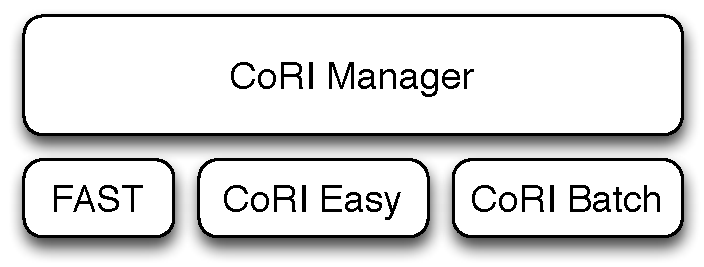
\includegraphics[scale=0.5]{fig/overviewCori}
    \caption{CoRI overview}
    \label{fig:cori-overview}
  \end{center}
\end{figure}

\subsection{Functions and tags}
The tags for information are of type \texttt{integer} and defined in the
table~\ref{t:tags}. The second type of tag \texttt{diet\_est\_collect\_tag\_t}
is used to specify which collector will provide the information:
\texttt{EST\_COLL\_EASY} or \texttt{EST\_COLL\_BATCH}.
Three different functions are provided with CoRI.

The first function initializes a specific collector.

\footnotesize
\begin{verbatim}
  int
  diet_estimate_cori_add_collector(diet_est_collect_tag_t collector_type,
                                   void * data);
\end{verbatim}
\normalsize The second parameter is reserved for initializing collectors which
need additional information on initialization. For example, the BATCH collector
needs for its initialization the profile of the service to be solved.

After the initialization, accessing to the information is done by specifying
the collector and the information type.
\footnotesize
\begin{verbatim}
  int
  diet_estimate_cori(estVector_t ev,
                     int info_type,
                     diet_est_collect_tag_t collector_type,
                     void* data);
\end{verbatim}
\normalsize

Cori-Easy doesn't need more information, but BATCH need a profile of
type ``diet\_profile\_t''. The last parameter is reserved for it. \\ The last
function is used to test Cori-Easy. It prints all information Cori-Easy finds
to the standard output.

\footnotesize
\begin{verbatim}
  void
  diet_estimate_coriEasy_print();
\end{verbatim}
\normalsize
A result could be the following output:
\footnotesize
\begin{verbatim}
start printing CoRI values..
cpu average load : 0.56
CPU 0 cache : 1024 Kb
number of processors : 1
CPU 0 Bogomips : 5554.17
diskspeed in reading : 9.66665 Mbyte/s
diskspeed in writing : 3.38776 Mbyte/s
total disk size : 7875.51 Mb
available disk size  :373.727 Mb
total memory : 1011.86 Mb
available memory : 22.5195 Mb
end printing CoRI values
\end{verbatim}
\normalsize

\subsection{CoRI-Easy}
The CoRI-Easy collector makes some basic system calls to gather the
information. CoRI-Easy is available by default. The last column of the
table~\ref{t:depcompil} corresponds to the CoRI-Easy's functionality.

There is an example on how to use CoRI-Easy in the
\verb!<diet_src>/src/examples/cori/! directory.

\subsection{CoRI batch}\label{section:cori_batch}

With the help of the CoRI batch collector, a \sed programmer can use some
information obtained from the batch system. It is only available if \diet is
compiled with the option \texttt{-DDIET\_USE\_BATCH} set to
\texttt{ON}. Currently, only simple information can be accessed but
functionalities will be improved along with the number of batch systems \diet
is able to address.

There is an example on how to use CoRI batch in
the\\ \verb!<diet_src>/src/examples/Batch/Cori_cycle_stealing/! directory.

\section{Future Work}

There are two primary efforts for the CoRI manager:
\begin{itemize}
\item \textbf{Improving CoRI-Easy}: Some evaluation functions are very basic
  and should be revised to increase their response time speed and the accuracy
  of the information. There is a need for other information (\ie information
  about the network). Every operating systems provide other basic functions to
  get the information. CoRI-Easy doesn't know all functions. Use the
  \texttt{diet\_estimate\_cori\_print()} function to test what CoRI-Easy can
  find on your \sed. Send us a mail if not  all functions are working properly.

\item \textbf{Improving CoRI batch}: add new functionalities to access dynamic
  information as well as some kind of performance predictions for more batch
  systems.

\item \textbf{New collectors}: Integrating other external tools like
  Ganglia~\cite{Ganglia} or Nagios~\cite{Nagios} to the CoRI Manager can
  provide more useful and exact information.
\end{itemize}

%%% Local Variables:
%%% mode: latex
%%% ispell-local-dictionary: "american"
%%% mode: flyspell
%%% fill-column: 79
%%% End:
